\documentclass[
  man,
  floatsintext,
  longtable,
  nolmodern,
  notxfonts,
  notimes,
  colorlinks=true,linkcolor=blue,citecolor=blue,urlcolor=blue]{apa7}

\usepackage{amsmath}
\usepackage{amssymb}



\usepackage[bidi=default]{babel}
\babelprovide[main,import]{english}


\babelfont{rm}[,RawFeature={fallback=mainfontfallback}]{Times New Roman}
% get rid of language-specific shorthands (see #6817):
\let\LanguageShortHands\languageshorthands
\def\languageshorthands#1{}

\RequirePackage{longtable}
\RequirePackage{threeparttablex}

\makeatletter
\renewcommand{\paragraph}{\@startsection{paragraph}{4}{\parindent}%
	{0\baselineskip \@plus 0.2ex \@minus 0.2ex}%
	{-.5em}%
	{\normalfont\normalsize\bfseries\typesectitle}}

\renewcommand{\subparagraph}[1]{\@startsection{subparagraph}{5}{0.5em}%
	{0\baselineskip \@plus 0.2ex \@minus 0.2ex}%
	{-\z@\relax}%
	{\normalfont\normalsize\bfseries\itshape\hspace{\parindent}{#1}\textit{\addperi}}{\relax}}
\makeatother




\usepackage{longtable, booktabs, multirow, multicol, colortbl, hhline, caption, array, float, xpatch}
\setcounter{topnumber}{2}
\setcounter{bottomnumber}{2}
\setcounter{totalnumber}{4}
\renewcommand{\topfraction}{0.85}
\renewcommand{\bottomfraction}{0.85}
\renewcommand{\textfraction}{0.15}
\renewcommand{\floatpagefraction}{0.7}

\usepackage{tcolorbox}
\tcbuselibrary{listings,theorems, breakable, skins}
\usepackage{fontawesome5}

\definecolor{quarto-callout-color}{HTML}{909090}
\definecolor{quarto-callout-note-color}{HTML}{0758E5}
\definecolor{quarto-callout-important-color}{HTML}{CC1914}
\definecolor{quarto-callout-warning-color}{HTML}{EB9113}
\definecolor{quarto-callout-tip-color}{HTML}{00A047}
\definecolor{quarto-callout-caution-color}{HTML}{FC5300}
\definecolor{quarto-callout-color-frame}{HTML}{ACACAC}
\definecolor{quarto-callout-note-color-frame}{HTML}{4582EC}
\definecolor{quarto-callout-important-color-frame}{HTML}{D9534F}
\definecolor{quarto-callout-warning-color-frame}{HTML}{F0AD4E}
\definecolor{quarto-callout-tip-color-frame}{HTML}{02B875}
\definecolor{quarto-callout-caution-color-frame}{HTML}{FD7E14}

%\newlength\Oldarrayrulewidth
%\newlength\Oldtabcolsep


\usepackage{hyperref}




\providecommand{\tightlist}{%
  \setlength{\itemsep}{0pt}\setlength{\parskip}{0pt}}
\usepackage{longtable,booktabs,array}
\usepackage{calc} % for calculating minipage widths
% Correct order of tables after \paragraph or \subparagraph
\usepackage{etoolbox}
\makeatletter
\patchcmd\longtable{\par}{\if@noskipsec\mbox{}\fi\par}{}{}
\makeatother
% Allow footnotes in longtable head/foot
\IfFileExists{footnotehyper.sty}{\usepackage{footnotehyper}}{\usepackage{footnote}}
\makesavenoteenv{longtable}

\usepackage{graphicx}
\makeatletter
\newsavebox\pandoc@box
\newcommand*\pandocbounded[1]{% scales image to fit in text height/width
  \sbox\pandoc@box{#1}%
  \Gscale@div\@tempa{\textheight}{\dimexpr\ht\pandoc@box+\dp\pandoc@box\relax}%
  \Gscale@div\@tempb{\linewidth}{\wd\pandoc@box}%
  \ifdim\@tempb\p@<\@tempa\p@\let\@tempa\@tempb\fi% select the smaller of both
  \ifdim\@tempa\p@<\p@\scalebox{\@tempa}{\usebox\pandoc@box}%
  \else\usebox{\pandoc@box}%
  \fi%
}
% Set default figure placement to htbp
\def\fps@figure{htbp}
\makeatother


% definitions for citeproc citations
\NewDocumentCommand\citeproctext{}{}
\NewDocumentCommand\citeproc{mm}{%
  \begingroup\def\citeproctext{#2}\cite{#1}\endgroup}
\makeatletter
 % allow citations to break across lines
 \let\@cite@ofmt\@firstofone
 % avoid brackets around text for \cite:
 \def\@biblabel#1{}
 \def\@cite#1#2{{#1\if@tempswa , #2\fi}}
\makeatother
\newlength{\cslhangindent}
\setlength{\cslhangindent}{1.5em}
\newlength{\csllabelwidth}
\setlength{\csllabelwidth}{3em}
\newenvironment{CSLReferences}[2] % #1 hanging-indent, #2 entry-spacing
 {\begin{list}{}{%
  \setlength{\itemindent}{0pt}
  \setlength{\leftmargin}{0pt}
  \setlength{\parsep}{0pt}
  % turn on hanging indent if param 1 is 1
  \ifodd #1
   \setlength{\leftmargin}{\cslhangindent}
   \setlength{\itemindent}{-1\cslhangindent}
  \fi
  % set entry spacing
  \setlength{\itemsep}{#2\baselineskip}}}
 {\end{list}}
\usepackage{calc}
\newcommand{\CSLBlock}[1]{\hfill\break\parbox[t]{\linewidth}{\strut\ignorespaces#1\strut}}
\newcommand{\CSLLeftMargin}[1]{\parbox[t]{\csllabelwidth}{\strut#1\strut}}
\newcommand{\CSLRightInline}[1]{\parbox[t]{\linewidth - \csllabelwidth}{\strut#1\strut}}
\newcommand{\CSLIndent}[1]{\hspace{\cslhangindent}#1}





\usepackage{fontspec} 

\defaultfontfeatures{Scale=MatchLowercase}
\defaultfontfeatures[\rmfamily]{Ligatures=TeX,Scale=1}

  \setmainfont[,RawFeature={fallback=mainfontfallback}]{Times New Roman}




\title{The Role of Race and Mental Illness Diagnosis on Stigmatization
of Homeless Individuals}


\shorttitle{STIGMA, HOMELESSNESS, MENTAL ILLNESS, AND RACE}


\usepackage{etoolbox}






\author{Karen Veronica Becerra}



\affiliation{
{Department of Psychology, The University of Chicago}}




\leftheader{Becerra}



\abstract{Homelessness in the United States is a persistent problem that
can have serious implications on the well-being of homeless individuals.
The present study focused on the role of race and mental illness
diagnosis on the stigmatization of homeless individuals, specifically
looking at the outcomes of the Attribution Questionnaire. This
questionnaire assessed the aspects of social distance, blame,
dangerousness, concern, and willingness to help of 215 participants
varying in ages across adulthood. The study was a self-paced online form
that used six experimental vignettes. The results indicated that there
were no significant interactions of race x diagnosis on stigmatization.
Additionally, race had no significant main effects, suggesting it was
not a significant factor for stigmatization of homeless individuals.
However, there were some significant main effects of diagnosis. Findings
might suggest that future work in reducing mental illness stigma and
increasing education could help decrease stigmatization of the homeless
population. }

\keywords{Homelessness, Stigmatization, Race, Mental
Illness, Diagnosis, Attribution Questionnaire}

\authornote{\par{\addORCIDlink{Karen Veronica
Becerra}{0009-0006-4967-0955}} 

\par{       }
\par{Correspondence concerning this article should be addressed to Karen
Veronica Becerra, Department of Psychology, The University of
Chicago, 5848 S. University
Avenue, Chicago, IL 60637, USA, Email: kvbecerra@uchicago.edu}
}

\makeatletter
\let\endoldlt\endlongtable
\def\endlongtable{
\hline
\endoldlt
}
\makeatother

\urlstyle{same}



\makeatletter
\@ifpackageloaded{caption}{}{\usepackage{caption}}
\AtBeginDocument{%
\ifdefined\contentsname
  \renewcommand*\contentsname{Table of contents}
\else
  \newcommand\contentsname{Table of contents}
\fi
\ifdefined\listfigurename
  \renewcommand*\listfigurename{List of Figures}
\else
  \newcommand\listfigurename{List of Figures}
\fi
\ifdefined\listtablename
  \renewcommand*\listtablename{List of Tables}
\else
  \newcommand\listtablename{List of Tables}
\fi
\ifdefined\figurename
  \renewcommand*\figurename{Figure}
\else
  \newcommand\figurename{Figure}
\fi
\ifdefined\tablename
  \renewcommand*\tablename{Table}
\else
  \newcommand\tablename{Table}
\fi
}
\@ifpackageloaded{float}{}{\usepackage{float}}
\floatstyle{ruled}
\@ifundefined{c@chapter}{\newfloat{codelisting}{h}{lop}}{\newfloat{codelisting}{h}{lop}[chapter]}
\floatname{codelisting}{Listing}
\newcommand*\listoflistings{\listof{codelisting}{List of Listings}}
\makeatother
\makeatletter
\makeatother
\makeatletter
\@ifpackageloaded{caption}{}{\usepackage{caption}}
\@ifpackageloaded{subcaption}{}{\usepackage{subcaption}}
\makeatother

% From https://tex.stackexchange.com/a/645996/211326
%%% apa7 doesn't want to add appendix section titles in the toc
%%% let's make it do it
\makeatletter
\xpatchcmd{\appendix}
  {\par}
  {\addcontentsline{toc}{section}{\@currentlabelname}\par}
  {}{}
\makeatother

%% Disable longtable counter
%% https://tex.stackexchange.com/a/248395/211326

\usepackage{etoolbox}

\makeatletter
\patchcmd{\LT@caption}
  {\bgroup}
  {\bgroup\global\LTpatch@captiontrue}
  {}{}
\patchcmd{\longtable}
  {\par}
  {\par\global\LTpatch@captionfalse}
  {}{}
\apptocmd{\endlongtable}
  {\ifLTpatch@caption\else\addtocounter{table}{-1}\fi}
  {}{}
\newif\ifLTpatch@caption
\makeatother

\begin{document}

\maketitle


\setcounter{secnumdepth}{-\maxdimen} % remove section numbering

\setlength\LTleft{0pt}


Homelessness in the United States and the struggle to give individuals
adequate housing is a persistent problem. Before the Covid -19 pandemic,
the number of homeless individuals was on the rise with 568,000
individuals experiencing homelessness in 2019, an increase of 15,000
from the previous
year(\citeproc{ref-frostHomelessnessWasRise2020}{Frost, 2020}). With the
current Covid-19 pandemic, we can only predict that those numbers have
continued to increase. In the United States, 2.4\% of homeless
individuals die each year (Stasha, 2020). We know that the general
population often tries to distance itself from the stigmatized
population, more specifically the homeless population. Homeless
individuals face greater stigma and social isolation and often are
removed from public parks and other locations because the general public
does not want them too close. The problems caused by stigmatization,
such as social distancing, can affect the homeless population in terms
of resources that they have available such as sanitation centers,
employment, and social support. Often the homeless population lacks
resources and is exposed to the elements which can increase their
mortality, as well as the chance of being malnourished, having parasitic
infestations, periodontal disease, degenerative joint diseases, venereal
diseases, cirrhosis, and hepatitis-related to intravenous (IV) drug
abuse. Public attitudes toward homeless individuals can influence
policies and the services provided to this population. The attitudes
displayed through the stigma of homeless individuals can have an impact
on both physical and psychological health and willingness to access
services. The impact of these stigmas has shown to have serious
implications on the well-being of homeless individuals. The present
study examined factors that could predict levels of stigmatization
expressed towards homeless individuals.

\subsection{Literature review}\label{literature-review}

Research on the stigma of mental illness, homelessness, and race
highlights its harmful effects on health and social integration. P. W.
Corrigan et al. (\citeproc{ref-corriganPublicStigmaMental2009}{2009})
examined public stigma, focusing on stereotypes like causal attribution
(blaming individuals for their condition) and dangerousness (perceiving
them as threatening). Using vignette-based experiments, the study found
that people with psychiatric disorders, especially those with drug
addiction, faced greater stigma than those with physical disabilities,
laying the foundation for understanding how schizophrenia and substance
use disorders contribute to homelessness stigma.

While P. Corrigan et al.
(\citeproc{ref-corriganAttributionModelPublic2003}{2003}) explored
mental illness stigma, it did not examine health outcomes. In contrast,
Weisz and Quinn
(\citeproc{ref-weiszStigmatizedIdentitiesPsychological2018}{2018})
demonstrated that homelessness stigma leads to psychological distress,
poor health, and social avoidance. Among 175 volunteers at a homeless
event, those experiencing or anticipating stigma reported worse physical
and mental health and greater reluctance to seek services. Participants
of color faced even higher distress and service avoidance, highlighting
the compounded impact of race and homelessness stigma.

Building on this, Markowitz and Syverson
(\citeproc{ref-markowitzRaceGenderHomelessness2021}{2021}) investigated
race and gender intersections in stigma. They found that black homeless
individuals were perceived as more dangerous than white counterparts,
though no significant differences in social distance emerged. However,
the study's reliance on college-aged participants, who may have been
more tolerant than the general population, was a limitation. The present
study addresses this by including a broader, more diverse sample.

Similarly, Gattis and Larson
(\citeproc{ref-gattisPerceivedRacialSexual2016}{2016}) linked racial
stigma and discrimination to heightened depression among 89 black
adolescents and young adults experiencing homelessness. Using social and
minority stress models, the study highlighted how marginalized groups
face greater psychological distress due to limited societal support.
Though constrained by a small sample, it reinforced the role of racial
stigma in homelessness experiences.

In sum, stigma related to homelessness, mental illness, and race
profoundly affects psychological and physical health, social
integration, and resource access. The present study expands on this
research by examining how mental illness and race interact to shape
stigma, offering a more nuanced understanding of its impact on homeless
individuals

\subsection{Current Study}\label{current-study}

Building on the research by P. W. Corrigan et al.
(\citeproc{ref-corriganPublicStigmaMental2009}{2009}), Markowitz and
Syverson (\citeproc{ref-markowitzRaceGenderHomelessness2021}{2021}), and
Weisz and Quinn
(\citeproc{ref-weiszStigmatizedIdentitiesPsychological2018}{2018}) the
current study aimed to explore how race and mental illness diagnosis
impact the stigmatization of homeless individuals. The research
specifically focused on mental illness, distinguishing between
individuals with schizophrenia and those with substance use disorders,
and examined how these factors interact with race in shaping stigma.
Previous studies suggest that public stigma varies across mental health
conditions and that race plays a crucial role in determining the
intensity of stigma. Based on these findings, the present study
hypothesized that race would significantly influence social distance,
perceived danger, blameworthiness, and emotional responses (concern and
help) toward homeless individuals. Specifically, it was predicted that
black homeless individuals would experience greater social distance, be
perceived as more dangerous and more blameworthy, and receive less
concern and help compared to their white counterparts. Additionally, it
was anticipated that individuals with substance use disorders would face
higher levels of social distance, dangerousness, and blame, while
individuals with schizophrenia would receive more concern and help.
Lastly, the study predicted that race and mental illness diagnosis would
interact to influence all aspects of stigmatization.

\subsubsection{Hypotheses}\label{hypotheses}

\paragraph{Effect of Race on
Stigmatization.}\label{effect-of-race-on-stigmatization}

\begin{quote}
\begin{enumerate}
\def\labelenumi{\arabic{enumi}.}
\tightlist
\item
  Black homeless individuals will experience greater social distance.
\item
  Black homeless individuals will be perceived as more dangerous.
\item
  Black homeless individuals will be perceived as more blameworthy.
\item
  Black homeless individuals will receive less concern and help compared
  to white homeless individuals.
\end{enumerate}
\end{quote}

\paragraph{Effect of Mental Illness Diagnosis on
Stigmatization.}\label{effect-of-mental-illness-diagnosis-on-stigmatization}

\begin{quote}
\begin{enumerate}
\def\labelenumi{\arabic{enumi}.}
\tightlist
\item
  Individuals with substance use disorders will face higher levels of
  social distance.
\item
  Individuals with substance use disorders will be perceived as more
  dangerous.
\item
  Individuals with substance use disorders will be perceived as more
  blameworthy.
\item
  Individuals with schizophrenia will receive more concern and help.
\item
  Interaction Between Race and Mental Illness Diagnosis
\end{enumerate}
\end{quote}

\paragraph{Race and mental illness diagnosis
interaction.}\label{race-and-mental-illness-diagnosis-interaction}

\begin{quote}
\begin{enumerate}
\def\labelenumi{\arabic{enumi}.}
\tightlist
\item
  Race and mental Illness diagnosis will interact to influence all
  aspects of stigmatization, including social distance, perceived
  danger, blameworthiness, concern, and willingness to help.
\end{enumerate}
\end{quote}

\section{Method}\label{method}

\subsection{Participants}\label{participants}

The sample for this study consisted of 215 participants, primarily
college-aged students in the United States, with ages ranging from The
ages of the sample ranged from 18 to 79 (M = 35.08, SD = 16.33).The
sample was 44.7\% White, 13\% Hispanic, 33\% Black, 4.2\% Asian
American, 3.3\% Biracial, and 1.9\% other ethnicities. The sample
identified politically as 52.6\% Liberal, 37.1\% Moderate, and 10.3\%
Conservative.The sample was broken down into 1.9\% living in a rural
community, 58.6\% living in the suburbs, 12.1\% living in a small town,
and 27.4\% living in a large metropolitan city. Finally, the
distribution of gender was as follows: 29.3\% male, 68.8\% female, and
1.9\% other responses. Table 1 provides a summary of the demographic
characteristics of the sample.

\subsubsection{Table 1}\label{table-1}

Demographic Information of Participants

\begin{longtable}[]{@{}ll@{}}
\toprule\noalign{}
\textbf{Demographic} & \textbf{Percentage} \\
\midrule\noalign{}
\endhead
\bottomrule\noalign{}
\endlastfoot
\textbf{Age (M = 35.08, SD = 16.33)} & - \\
\textbf{Ethnicity} & \\
White & 44.7\% \\
Hispanic & 13\% \\
Black & 33\% \\
Asian American & 4.2\% \\
Biracial & 3.3\% \\
Other Ethnicities & 1.9\% \\
\textbf{Political Affiliation} & \\
Liberal & 52.6\% \\
Moderate & 37.1\% \\
Conservative & 10.3\% \\
\textbf{Location} & \\
Rural Community & 1.9\% \\
Suburbs & 58.6\% \\
Small Town & 12.1\% \\
Large Metropolitan City & 27.4\% \\
\textbf{Gender} & \\
Male & 29.3\% \\
Female & 68.8\% \\
Other Responses & 1.9\% \\
\end{longtable}

\textbf{Note}: Percentages may not sum to 100 due to rounding.

\subsection{Measures}\label{measures}

This study used multiple questionnaires to examine the effects and
interactions of race and mental illness on stigmatization toward
homeless individuals. Participants were assigned to one of six
experimental conditions using vignettes adapted from Markowitz and
Syverson (\citeproc{ref-markowitzRaceGenderHomelessness2021}{2021}),
manipulating race and mental illness. Table 2 presents the vignettes
used in this study.

\subsubsection{Table 2}\label{table-2}

Vignettes Used in the Study

\begin{longtable}[]{@{}
  >{\raggedright\arraybackslash}p{(\linewidth - 6\tabcolsep) * \real{0.3673}}
  >{\raggedright\arraybackslash}p{(\linewidth - 6\tabcolsep) * \real{0.0816}}
  >{\raggedright\arraybackslash}p{(\linewidth - 6\tabcolsep) * \real{0.1769}}
  >{\raggedright\arraybackslash}p{(\linewidth - 6\tabcolsep) * \real{0.3741}}@{}}
\toprule\noalign{}
\begin{minipage}[b]{\linewidth}\raggedright
\textbf{Condition}
\end{minipage} & \begin{minipage}[b]{\linewidth}\raggedright
\textbf{Race}
\end{minipage} & \begin{minipage}[b]{\linewidth}\raggedright
\textbf{Mental Illness}
\end{minipage} & \begin{minipage}[b]{\linewidth}\raggedright
\textbf{Character Description}
\end{minipage} \\
\midrule\noalign{}
\endhead
\bottomrule\noalign{}
\endlastfoot
Condition 1: Black character/No mental illness & Black & No mental
illness & Male homeless individual with same life story \\
Condition 2: Black character/Substance use disorder & Black & Substance
use disorder & Male homeless individual with same life story \\
Condition 3: Black character/Schizophrenia & Black & Schizophrenia &
Male homeless individual with same life story \\
Condition 4: White character/No mental illness & White & No mental
illness & Male homeless individual with same life story \\
Condition 5: White character/Substance use disorder & White & Substance
use disorder & Male homeless individual with same life story \\
Condition 6: White character/Schizophrenia & White & Schizophrenia &
Male homeless individual with same life story \\
\end{longtable}

\textbf{Note:} All vignettes used the same life story for the male
homeless individual, with only race and mental illness varying across
conditions.

\subsubsection{Attribution
Questionnaire}\label{attribution-questionnaire}

The Attribution
Questionnaire(\citeproc{ref-corriganAttributionModelPublic2003}{P.
Corrigan et al., 2003}) assessed stigmatization aspects like social
distance, blame, perceived dangerousness, emotional response, and
willingness to help.

\subsubsection{Memory Check}\label{memory-check}

A Memory Check assessed participants' recall of story details,
specifically the race and mental illness of the character.

\subsubsection{Demographic
Questionnaire}\label{demographic-questionnaire}

Demographics questionnaire that asked participants about their age,
ethnicity, residence, political affiliation, and familiarity with
homelessness.

\section{Results}\label{results}

\subsection{MAin Effect of Diagnosis on Social Distance
Stigma}\label{main-effect-of-diagnosis-on-social-distance-stigma}

\begin{figure}[!htbp]

{\caption{{Effect of Mental Illness Diagnosis on Social Distance
Stigma.}{\label{fig-social-distance-stigma}}}}

\pandocbounded{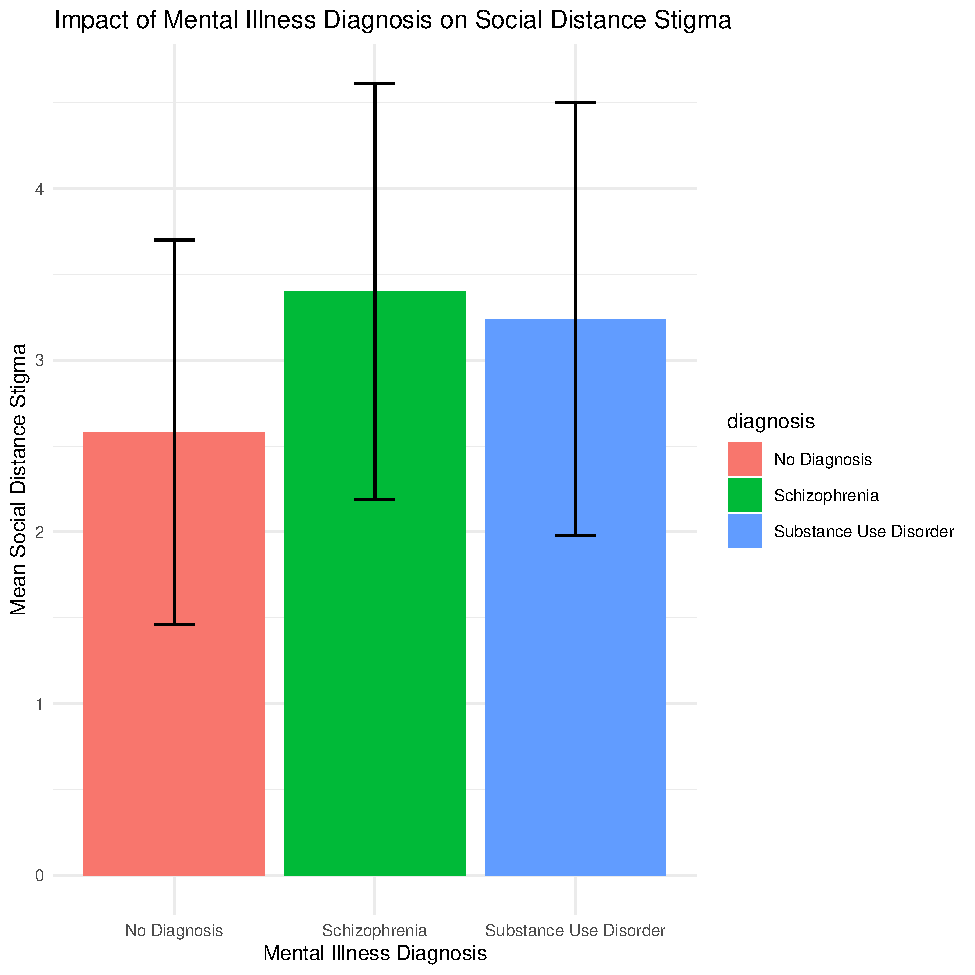
\includegraphics[keepaspectratio]{The-Role-of-Race-and-Mental-Illness-Diagnosis-on-Stigmatization-of-Homeless-Individuals_files/figure-pdf/fig-social-distance-stigma-1.pdf}}

{\noindent \emph{Note.} The plot shows mean social distance stigma
scores by diagnosis, with error bars representing standard deviation.}

\end{figure}

Figure 1 shows the effect of mental illness diagnosis on social distance
stigma. The mean stigma scores for each diagnosis are as follows:No
Diagnosis: 2.58 (SD = 1.12), Schizophrenia: 3.4 (SD = 1.21),Substance
Use Disorder: 3.24 (SD = 1.26)

The results indicate that individuals with schizophrenia (M = 3.4) and
substance use disorder (M = 3.24) experience higher levels of social
distance stigma compared to those with no diagnosis (M = 2.58). However,
these differences were not statistically significant.

\section{Discussion}\label{discussion}

This study examined the role of race and mental illness diagnosis in the
stigmatization of homeless individuals, using the Attribution
Questionnaire to measure social distance, blame, dangerousness, concern,
and willingness to help. We hypothesized that race would significantly
impact all aspects of stigmatization, with Black homeless individuals
receiving more negative perceptions. However, none of these predictions
were supported, as race did not significantly affect the levels of
stigmatization. These findings align with some previous studies but
contradict others, particularly regarding perceived dangerousness, where
Black individuals were not viewed as more dangerous than White
individuals.

Regarding mental illness, we predicted that substance use disorders
would result in higher social distance, dangerousness, and blame, while
schizophrenia would lead to more concern and help. While there was no
significant effect for help and concern, individuals with schizophrenia
were perceived as more dangerous and socially distant, contrary to prior
research. Substance use disorder diagnosis was associated with higher
levels of blame, suggesting a stronger stigmatization of this group.

Regarding interactions between race and mental illness, we predicted
that Black homeless individuals with substance use disorders would
receive the highest levels of stigma. However, no significant
interaction was found. These results suggest that mental illness
diagnosis plays a larger role in stigmatization than race.

The study had limitations, including an online format that may have
influenced responses due to social pressure, and a sample largely
composed of college-aged students and liberals, which could affect the
generalizability of the findings. Future research should include a more
diverse sample and consider factors such as desirability and response
truthfulness.

\section{References}\label{references}

\phantomsection\label{refs}
\begin{CSLReferences}{1}{0}
\bibitem[\citeproctext]{ref-corriganPublicStigmaMental2009}
Corrigan, P. W., Kuwabara, S. A., \& O'Shaughnessy, J. (2009). The
{Public Stigma} of {Mental Illness} and {Drug Addiction}: {Findings}
from a {Stratified Random Sample}. \emph{Journal of Social Work},
\emph{9}(2), 139--147. \url{https://doi.org/10.1177/1468017308101818}

\bibitem[\citeproctext]{ref-corriganAttributionModelPublic2003}
Corrigan, P., Markowitz, F. E., Watson, A., Rowan, D., \& Kubiak, M. A.
(2003). An {Attribution Model} of {Public Discrimination Towards
Persons} with {Mental Illness}. \emph{Journal of Health and Social
Behavior}, \emph{44}(2), 162. \url{https://doi.org/10.2307/1519806}

\bibitem[\citeproctext]{ref-frostHomelessnessWasRise2020}
Frost, R. (2020). \emph{Homelessness {Was} on the {Rise}, {Even} before
the {Pandemic} {\textbar} {Joint Center} for {Housing Studies}.}

\bibitem[\citeproctext]{ref-gattisPerceivedRacialSexual2016}
Gattis, M. N., \& Larson, A. (2016). Perceived racial, sexual identity,
and homeless status-related discrimination among {Black} adolescents and
young adults experiencing homelessness: {Relations} with depressive
symptoms and suicidality. \emph{American Journal of Orthopsychiatry},
\emph{86}(1), 79--90. \url{https://doi.org/10.1037/ort0000096}

\bibitem[\citeproctext]{ref-markowitzRaceGenderHomelessness2021}
Markowitz, F. E., \& Syverson, J. (2021). Race, {Gender}, and
{Homelessness Stigma}: {Effects} of {Perceived Blameworthiness} and
{Dangerousness}. \emph{Deviant Behavior}, \emph{42}(7), 919--931.
\url{https://doi.org/10.1080/01639625.2019.1706140}

\bibitem[\citeproctext]{ref-weiszStigmatizedIdentitiesPsychological2018}
Weisz, C., \& Quinn, D. M. (2018). Stigmatized identities, psychological
distress, and physical health: {Intersections} of homelessness and race.
\emph{Stigma and Health}, \emph{3}(3), 229--240.
\url{https://doi.org/10.1037/sah0000093}

\end{CSLReferences}






\end{document}
